\documentclass[a4paper,12pt,oneside,openany,table,xcdraw]{article}

\usepackage{setspace}
\usepackage{multirow}
\usepackage{hyperref}
\usepackage{caption}
\usepackage{indentfirst}

\usepackage[brazilian]{babel}
\usepackage[utf8x]{inputenc}
\usepackage{amsmath, graphicx, mathptmx, enumerate}
\usepackage{float}
\usepackage[colorinlistoftodos]{todonotes}
\usepackage{makeidx} % Para o sumário
\usepackage{geometry}

\geometry{a4paper, hmargin={3cm, 3cm}, vmargin={3cm, 2cm} }
\setlength{\parindent}{1.0cm}

\begin{document}
\newcommand{\thedepartment}{Faculdade de Engenharia Elétrica}
\newcommand{\thecourse}{FEELT}
\newcommand{\thetitle}{CIRCUITOS ACOPLADOS MAGNETICAMENTE}
\newcommand{\thetype}{Relatório da Disciplina de Circuitos Elétricos II}
\newcommand{\theproftitle}{Bacharel em Engenharia Elétrica}
\newcommand{\thestudent}{Lesly Viviane Montúfar Berrios\\
\centering11811ETE001}
\newcommand{\theadvisor}{Prof. Wellington Maycon Santos Bernardes}
\newcommand{\thecity}{Uberlândia}

\thispagestyle{empty}\newcommand*{\themonth}{\ifthenelse{\the\month < 2}{Janeiro }
                  {\ifthenelse{\the\month < 3}{Fevereiro }
                  {\ifthenelse{\the\month < 4}{Março }
                  {\ifthenelse{\the\month < 5}{Abril }
                  {\ifthenelse{\the\month < 6}{Maio }
                  {\ifthenelse{\the\month < 7}{Junho }
                  {\ifthenelse{\the\month < 8}{Julho }
                  {\ifthenelse{\the\month < 9}{Agosto }
                  {\ifthenelse{\the\month < 10}{Setembro }
                  {\ifthenelse{\the\month < 11}{Outubro }
                  {\ifthenelse{\the\month < 12}{Novembro }{Dezembro }}}}}}}}}}}}
                  
\begin{titlepage}
\begin{center}

	\vspace{-0.5cm}

  \begin{figure}[hbt!]
		\begin{center}
		   
\includegraphics[width=2.8cm]{ufu-logo.png}
		\end{center}
	\end{figure}
 	%\vspace{-4cm}

%\begin{doublespacing}

  \Large{\textbf{Universidade Federal de Uberlândia}}\\
  \large{\thedepartment}\\
  \large{\thecourse}\\


\vspace{5.8cm}
  \par
  \large\textbf{\thetitle}
\vspace{5.8cm} 

%\end{doublespacing}
  \par
  \thetype\\
  por\\
  %\hspace{2cm}\large{}\\

\vspace{0.8cm}
\par
  \normalsize{\thestudent}\\ [2cm]
  \theadvisor

\par\vfill
  \thecity, \themonth / \the\year

\end{center}

\end{titlepage}

%% Comeca o documento !

\onehalfspacing
\tableofcontents % sumário
\newpage

\section{Objetivos} % 2,5%
Verificar experimentalmente os conceitos teóricos sobre acoplamentos magnéticos,
obtenção dos valores das auto-indutâncias e da indutância mútua, e comparar os resultados
com os valores obtidos utilizando uma análise teórica.

\section{Introdução teórica} % 5%
Nos circuitos em que a condução de energia elétrica ocorre por meios físicos, diz-se que são circuitos condutivos. Entretanto, ainda é possível que dois circuitos com ou sem contato se afetem por meio do campo magnético gerado por um deles, esses são chamados circuitos magneticamente acoplados \cite{ph}.

O \emph{transformador} é baseado nesse princípio. Possui quatro terminais e consiste em dois indutores que são colocados com certa proximidade um do outro, logo comparttilham o mesmo fluxo magnético e, portanto, as bobinas indutoras estão acopladas magneticamente. 

É vasta a aplicabilidade desse equipamento, por exemplo, em sistemas de comunicação eles são usados para casamento de impedâncias entre fontes e cargas ou linhas de transmissão. Em sistemas de potências, transformadores são usados para atenuar ou amplificar os sinais de tensão. De fato, transformadores são utilizados em eliminadores de pilha e recarregadores de baterias, que podem ser ligados diretamente em tomadas residenciais \cite{irwin}.


\section{Preparação}
\subsection{Materiais e ferramentas} % 2,5%
\begin{enumerate}[1 - ]
\item \emph{Fonte}\\
Alimentará todo o circuito.

\item \emph{Conjunto de bobinas}\\
Cada bobina possui uma resistência, sendo $R_1$ para a Bobina 1 e $R_2$ para a Bobina 2. Considere $R_1\leq R_2$.

\item \emph{Conectores}\\
Foram utilizadas pontas de provas para a verificação das grandezas nos multímetros. Para as conexões no circuito foi utilizado majoritariamente cabos banana-banana.

\item \emph{Multímetro}\\
Utilizado para medir as tensões elétricas entre os pontos das bobinas especificados no experimento.

\item \emph{Miliamperímetro}\\
A escala mais precisa permite melhor regulagem da corrente desejada.

\item \emph{Varivolt}\\
O equipamento permitirá obter o valor desejado de corrente a partir da regulagem correta da tensão fornecida pela fonte.


\end{enumerate}

\subsection{Montagem} % 2,5%
\begin{enumerate}[1)]
\item \emph{Resistências das bobinas}\\
Para o conjunto de bobinas fornecido, foi medido a resistência da bobina 1 (600 esp.) e a
resistência da bobina 2 (1200 esp.) e obteve-se: 
$$R_1= 2,6$$ e $$R_2=7,4$$

\item \emph{Determinando a polaridade das bobinas}\\
Efetue a montagem da Figura \ref{2.2}, aplicando uma corrente de 50 mA no
miliamperímetro, anote a tensão V1 e marque a
polaridade da bobina 1, indicando-a por um ponto “.”, no terminal em que a fem1 (terminal
ligado ao positivo da fonte CA) é positiva. Na bobina 2 marque a polaridade ( o ponto ) no
terminal ligado ao voltímetro se a tensão V’ for menor que a tensão V1, e marque o ponto no
terminal debaixo se V’ for maior que V1 ( terminal em que a fem induzida é positiva). Anote
o esquema e o ponto no caderno.


\begin{figure}[!htb]
\centering
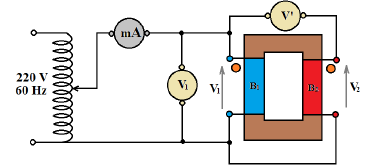
\includegraphics{fig1}
\caption{Marcação de polaridade}
\label{2.2}
\end{figure}


\end{enumerate}

\section{Análise sobre segurança} % 2,5%
Os óculos de segurança são Equipamentos de Proteção Individual (EPIs) e são utilizados para a proteção da área ao redor dos olhos contra qualquer tipo de detrito estranho, que possa causar irritação ou ferimentos. Também protegem contra faíscas, respingos de produtos químicos, detritos, poeira, radiação e etc \cite{safe}.
É importante a utilização desse equipamento durante os experimentos a fim de evitar qualquer dano, além de preparar o profissional para o manejo correto e seguro dos equipamentos.

\section{Cálculos, análise dos resultados e questões} %(quando houver) (70%)


\section{Simulação computacional} %(10%);

\section{Conclusões} % (no mínimo 10 linhas) (5%)


\newpage
\begin{thebibliography}{9} 
% Introdução
\bibitem{ph}
    P. H. Rezende,
    “Circuitos Magneticamente Acoplados”, UFU, 2018.
 Disponível em:
 \url{https://www.moodle.ufu.br/pluginfile.php/702496/mod_resource/content/3/Cap.\%20I_Acoplamento.pdf}. Acesso em: ago. 2019.

\bibitem{irwin}
    J. D. Irwin,
    “Análise de Circuitos Em Engenharia”, Pearson, $4^a$ Ed., 2000.


\bibitem{safe}
    SafetyTrabi,
    “Óculos de segurança: Saiba quando utilizar este EPI”, SafetyTrab, 2019.
 Disponível em:
 \url{https://www.safetytrab.com.br/blog/oculos-de-seguranca/}. Acesso em: ago. 2019.




\end{thebibliography}
\end{document}